\documentclass[a4paper,12pt]{article}
\usepackage[utf8]{inputenc}
\usepackage{hyperref}
\usepackage{graphicx}
\usepackage{float}
\graphicspath{ {images/} }

\begin{document}

\begin{titlepage}

\newcommand{\HRule}{\rule{\linewidth}{0.5mm}} % Defines a new command for the horizontal lines, change thickness here

\center % Center everything on the page
 
%----------------------------------------------------------------------------------------
%-	HEADING SECTIONS
%----------------------------------------------------------------------------------------	
\vfill
\textsc{\LARGE University of Pretoria}\\[1.5cm]
\textsc{\Large COS 301 - Software Engineering}\\[0.5cm]
\textsc{\large The Savage Ru's}\\[0.5cm]

%----------------------------------------------------------------------------------------
%-	TITLE SECTION
%----------------------------------------------------------------------------------------

\HRule \\[0.4cm]
{ \huge \bfseries VizARD Architectural and Functional Specification - Version 1}\\[0.4cm] % Title of your document
{\large \today}
\HRule \\[1.5cm]
 
%----------------------------------------------------------------------------------------
%-	AUTHOR SECTION
%----------------------------------------------------------------------------------------

\begin{minipage}{0.4\textwidth}
\begin{flushleft} \large
\emph{Author(s):}\\
Jodan \textsc{Alberts}\\ % Your name
Mark \textsc{Klingenberg}\\
Una \textsc{Rambani}\\
Ruan \textsc{Klinkert}\\
\end{flushleft}
\end{minipage}
~
\begin{minipage}{0.4\textwidth}
\begin{flushright} \large
\emph{Student number(s):} \\
14395283\\ % Student number
14020272\\
14004489\\
14022282\\

\end{flushright}
\end{minipage}\\[0.5cm]


\centering
	
\includegraphics[width=60mm]{SavageRu.jpg}

{\large \today}\\[3cm] % Date, change the \today to a set date if you want to be precise

\centering
	\textsc{\LARGE Epi-Use Labs project}\\[0.5cm]
	\textsc{\Large VizARD}\\[0.5cm]
	\textsc{\Large  Architectural and Functional Specification Version 1}\\[0.5cm]
	
\includegraphics[width=\textwidth]{images/vizard.png}
 % Date, change the \today to a set date if you want to be precise

 
%----------------------------------------------------------------------------------------

\vfill % Fill the rest of the page with whitespace

\end{titlepage}

\newpage

\tableofcontents

\newpage

\section{Introduction}

This is the software requirements specification for the vizARD Augmented Reality application that is being developed for EPI-USE Labs.
\newline
VizARD is a mobile application that allows for quick and easy visualization of tabular data.

\section{Vision and Background}
The system will allow a user to:
\begin{itemize}
\item Take a picture of a table of numerical data
\item Use OCR (Optical Character Recognition) to read the data from the picture
\item Generate an appropriate graph for the data
\item View a 3D model of this graph through Augmented Reality.
\end{itemize} 

\newpage
\section{Software Architecture}
\subsection{Architectural Scope}
ViZARD is a partially online application, since the OCR processing takes place on a remote server. After an image has been taken by the user, it is sent via a POST request to the OpenOCR API server for Tesseract to process. The results are returned and parsed into a C\# object where our scripts handle the graph generation.

\subsection{Integration and Access Channel Requirements}
\begin{itemize}
\item Each local deployment accesses the OpenOCR server through a RESTful API, which requires internet access.
\item  Since the application is being developed entirely in Unity3D (save for the OCR), Unity selects the APIs to complete tasks such as file system access, camera access and network access.
\item End users will be able to access the system through mobile applications made available for Android and iOS operating systems.
\end{itemize}

\subsection{Quality Requirements}
\subsubsection*{Usability}
\begin{itemize}		
	\item Generated graphs should be mapped on to the correct surface in the appropriate orientation
	\item Generated graphs should be scaled correctly, they should be stable and visible on the screen
\end{itemize}
\subsubsection*{Performance}	
\begin{itemize}		
	\item Data extraction from the images and graph generation should take a maximum of 10 seconds
	\item The application has to be responsive, that is, the application should react to touch within a second so that no lag is apparent.
	\item OCR data should be returned within 5 seconds of the image being sent to server, provided that internet speeds are greater than 2 mbps.	
\end{itemize}
\subsubsection*{Reliability}	
\begin{itemize}		
	\item The camera resolution should not be less than the screen resolution to ensure that accurate OCR analysis is achieved
\end{itemize}

\subsection{Architecture Constraints}
\begin{itemize}
	\item Android
	\item iOS
\end{itemize}
The systems used must be compatible with both iOS and Android.
\newline
To allow for this, the VizARD application will be developed in Unity 3D as a largely C\# based program. Through Unity's built in tools we will be able to build to the two required platforms more easily. 

\subsection{Architectural Patterns or Styles}
The system employs a derivation of MVC called MVP (Model View Presenter).
These MVP segments are as follows:
\begin{itemize}
	\item \textbf{Model -} this is the data access layer. In our case this is simply the device's file system API and the remote OCR server.
	\item\textbf{View -} this is the layer that displays information to the user and reacts to user input. The Unity Scenes that we have developed will serve this function.
	\item \textbf{Presenter -} the Presenter handles the background tasks such as sending and receiving data to and from the Model and View. In the case of VizARD, the Presenter consists mainly of the inner components of the Unity game engine.
	

We have decided to use this architectural pattern due to its pluggability and maintainability. By separating the system into these components we make troubleshooting and problem solving simpler.
\end{itemize}

\subsection{Technologies}
The application has 3 basic functions across 4 components:
\begin{itemize}
	\item Data Extraction from images - through OCR and user input using the Tesseract based OpenOCR server.
	\item Graph Generation - by using Unity 3D.
	\item Augmented Reality - through Vuforia AR SDK .
	\item User Interface - also built within Unity 3D and consists of Scripts and Scenes.	
\end{itemize}

\newpage
\section{Functional requirements and application design}
\subsection{Global Scope}
\begin{figure}[H]
		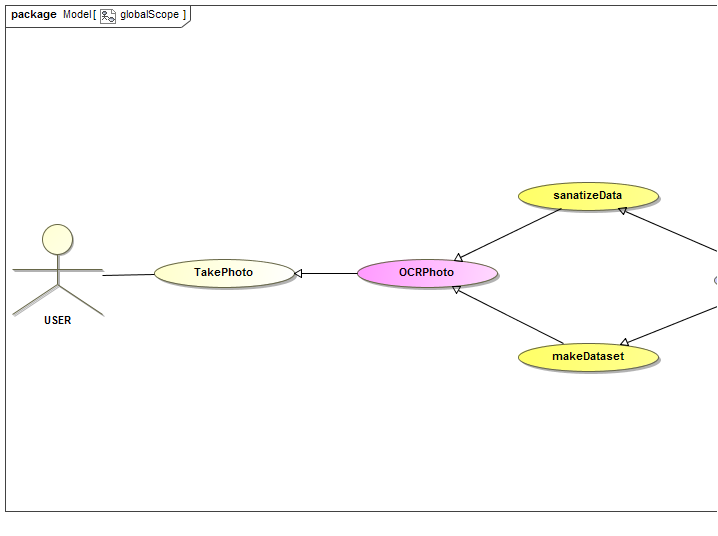
\includegraphics[width=\textwidth]{Images/globalScope.png}  \\
		\caption{Use Case: Global Scope}
	\end{figure}
	\begin{figure}[H]
		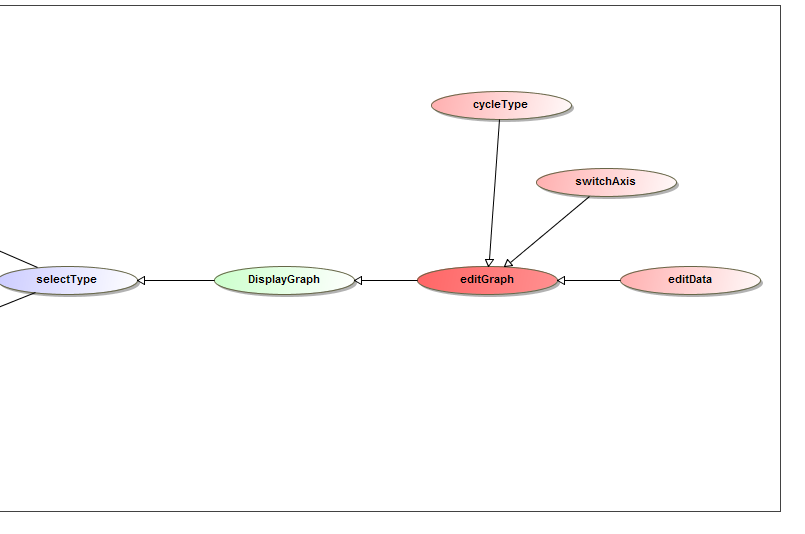
\includegraphics[width=\textwidth]{Images/globalscope2.png}  \\
		\caption{Use Case: Global Scope continued}
	\end{figure}
\subsection{Service contracts/Use Cases}
	\begin{figure}[H]
		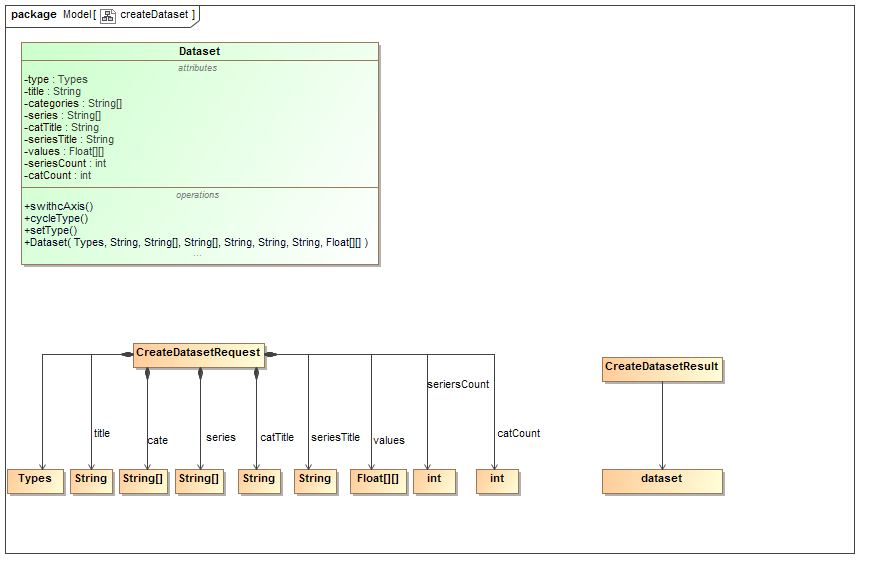
\includegraphics[width=\textwidth]{Images/createDataset.png}  \\
		\caption{Services Contract : createDataset}
	\end{figure}
	\begin{figure}[H]
		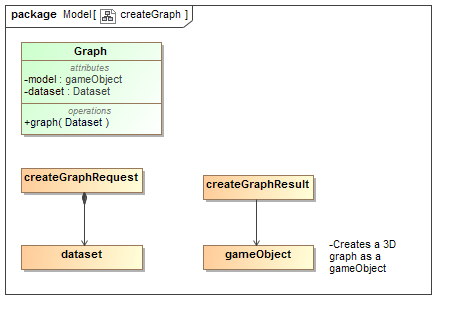
\includegraphics[width=\textwidth]{Images/createGraph.png}  \\
		\caption{Services Contract : createGraph}
	\end{figure}
	\begin{figure}[H]
		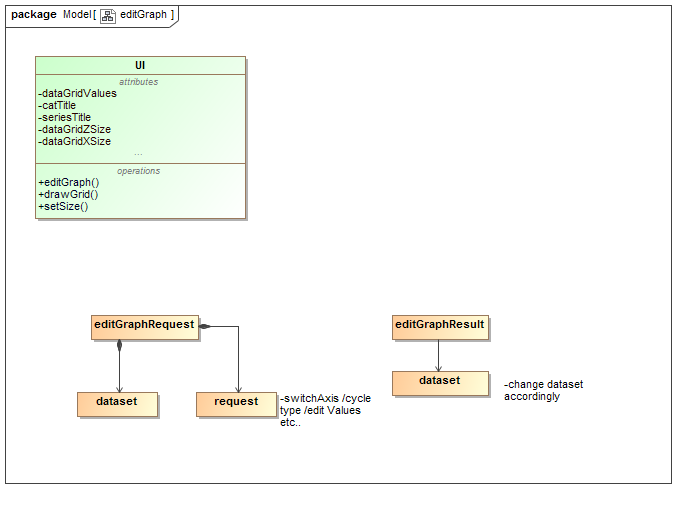
\includegraphics[width=\textwidth]{Images/editGraph.png}  \\
		\caption{Services Contract : editGraph}
	\end{figure}
	
	\begin{figure}[H]
		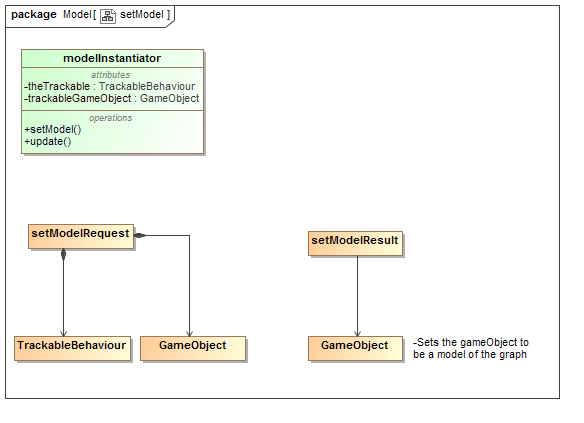
\includegraphics[width=\textwidth]{Images/setModel.png}  \\
		\caption{Services Contract : setModel}
	\end{figure}
	
	\begin{figure}[H]
		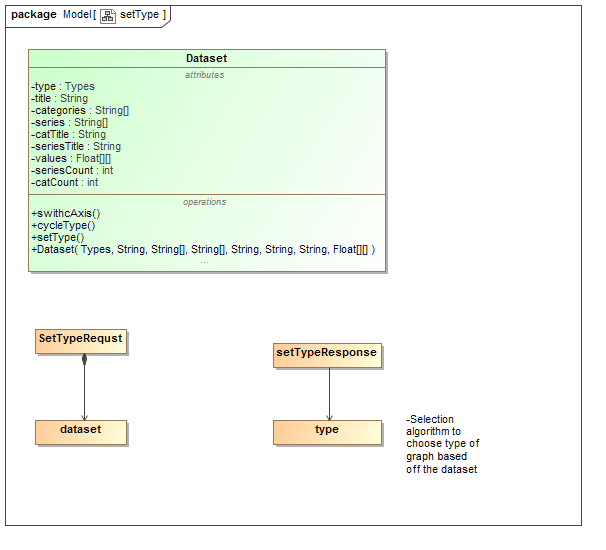
\includegraphics[width=\textwidth]{Images/setType.png}  \\
		\caption{Services Contract : setType}
	\end{figure}
	
	\begin{figure}[H]
		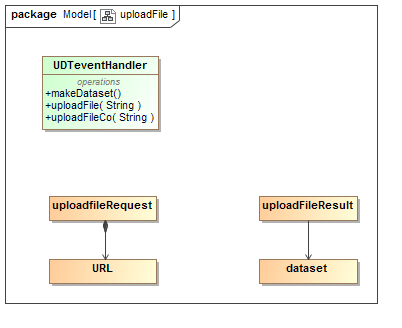
\includegraphics[width=\textwidth]{Images/uploadFile.png}  \\
		\caption{Services Contract : uploadFile}
	\end{figure}
	
	\begin{figure}[H]
		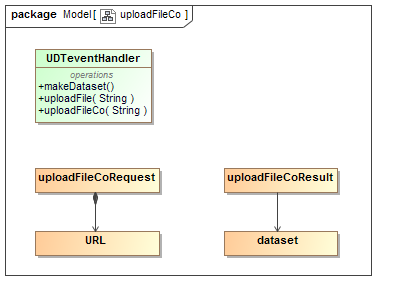
\includegraphics[width=\textwidth]{Images/uploadFileCo.png}  \\
		\caption{Services Contract : uploadFile co-routine}
	\end{figure}
	
\subsection{Required functionality}
	\begin{figure}[H]
		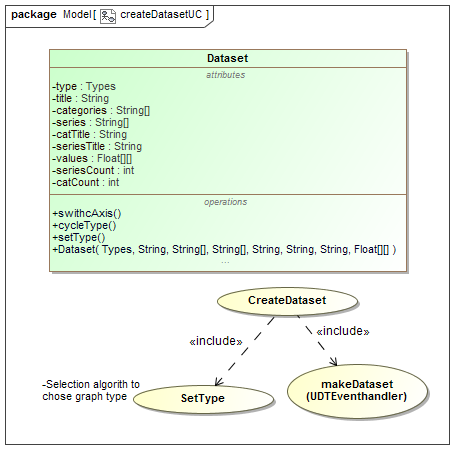
\includegraphics[width=\textwidth]{Images/createDatasetUC.png}  \\
		\caption{Required functionality : createDataset}
	\end{figure}
	\begin{figure}[H]
		\includegraphics[width=\textwidth]{Images/creategraphUC.png}  \\
		\caption{Required functionality : creategraph}
	\end{figure}
	\begin{figure}[H]
		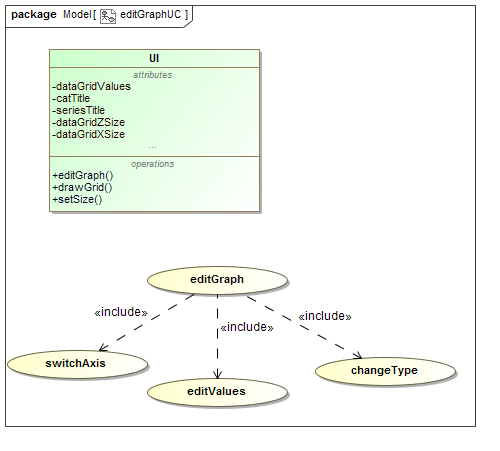
\includegraphics[width=\textwidth]{Images/editGraphUC.png}  \\
		\caption{Required functionality : editGraph}
	\end{figure}
	\begin{figure}[H]
		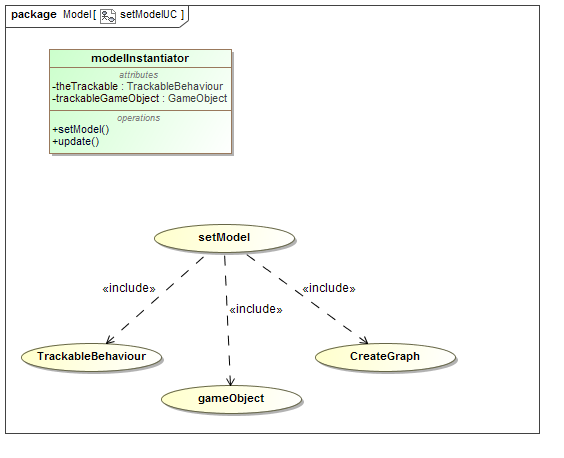
\includegraphics[width=\textwidth]{Images/setModelUC.png}  \\
		\caption{Required functionality : setModel}
	\end{figure}	
	
	\begin{figure}[H]
		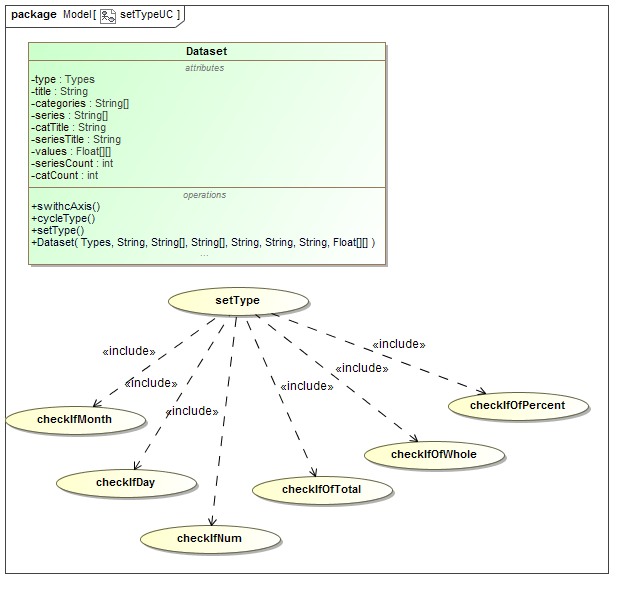
\includegraphics[width=\textwidth]{Images/setTypeUC.png}  \\
		\caption{Required functionality : setType}
	\end{figure}
	
	\begin{figure}[H]
		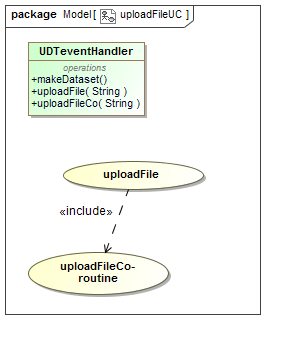
\includegraphics[width=\textwidth]{Images/uploadFileUC.png}  \\
		\caption{Required functionality : uploadFile}
	\end{figure}
	
	\begin{figure}[H]
		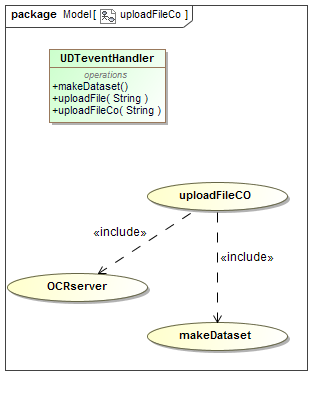
\includegraphics[width=\textwidth]{Images/uploadFileCoUC.png}  \\
		\caption{Required functionality : uploadFile co-routine}
	\end{figure}

\subsection{Activity Diagrams}

\begin{figure}[H]
		\includegraphics[width=\textwidth]{Images/createGraph__act.png}  \\
		\caption{Activity Diagram : createGraph}
	\end{figure}

\begin{figure}[H]
		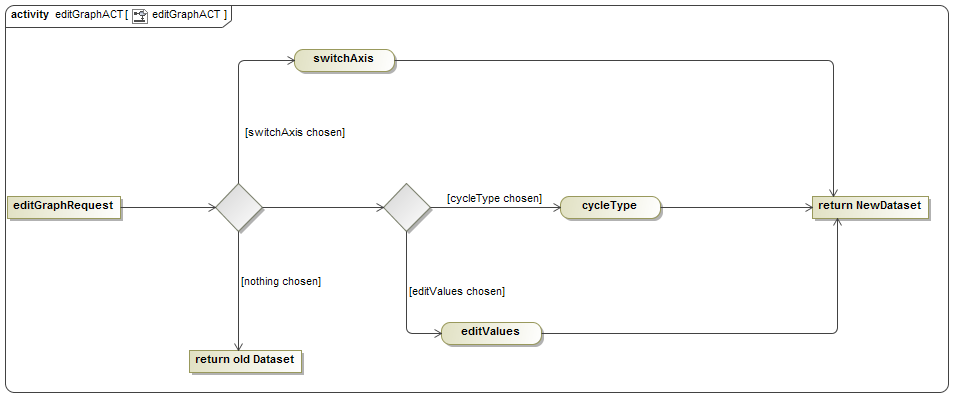
\includegraphics[width=\textwidth]{Images/editGraphACT.png}  \\
		\caption{Activity Diagram : editGraph}
	\end{figure}
	
\begin{figure}[H]
		\includegraphics[width=\textwidth]{Images/setModelACT.png}  \\
		\caption{Activity Diagram : setModel}
	\end{figure}
	
\begin{figure}[H]
		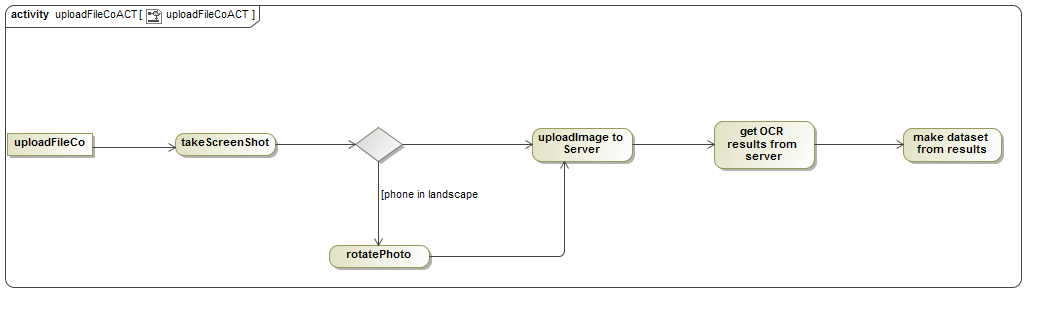
\includegraphics[width=\textwidth]{Images/uploadFileCoACT.png}  \\
		\caption{Activity Diagram :  uploadFile co-routine}
	\end{figure}
%\subsection{Domain Model}

%\subsection{Use of Reference Architectures and Frameworks}

%\subsubsection{Web 2.0 Reference Architecture}

%\subsection{Access and Integration Channels}

\newpage

\end{document}